\hypertarget{fca_8h}{\section{src/fca/fca.h \-File \-Reference}
\label{fca_8h}\index{src/fca/fca.\-h@{src/fca/fca.\-h}}
}


\hyperlink{fca_8h}{fca.\-h}, (c) 2013, \-Immanuel \-Albrecht; \-Dresden \-University of \-Technology, \-Professur für die \-Psychologie des \-Lernen und \-Lehrens  


{\ttfamily \#include \char`\"{}easy.\-h\char`\"{}}\*
{\ttfamily \#include \char`\"{}vector.\-h\char`\"{}}\*
\-Include dependency graph for fca.\-h\-:\nopagebreak
\begin{figure}[H]
\begin{center}
\leavevmode
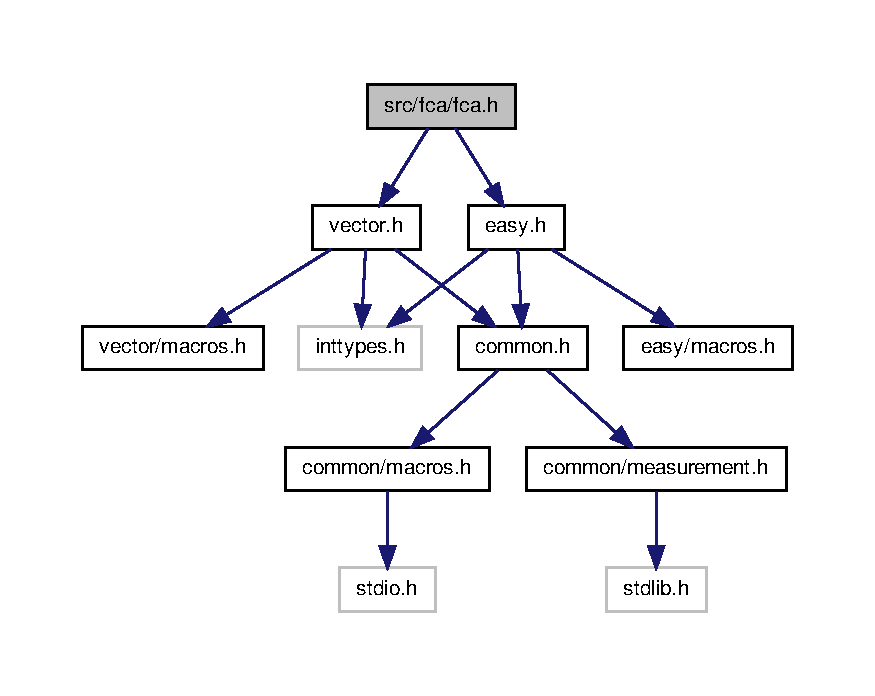
\includegraphics[width=350pt]{fca_8h__incl}
\end{center}
\end{figure}
\-This graph shows which files directly or indirectly include this file\-:\nopagebreak
\begin{figure}[H]
\begin{center}
\leavevmode
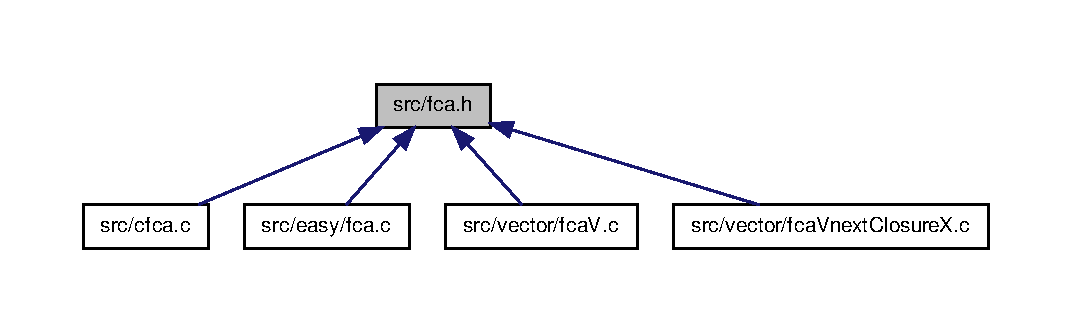
\includegraphics[width=150pt]{fca_8h__dep__incl}
\end{center}
\end{figure}


\subsection{\-Detailed \-Description}
\hyperlink{fca_8h}{fca.\-h}, (c) 2013, \-Immanuel \-Albrecht; \-Dresden \-University of \-Technology, \-Professur für die \-Psychologie des \-Lernen und \-Lehrens \-This program is free software\-: you can redistribute it and/or modify it under the terms of the \-G\-N\-U \-General \-Public \-License as published by the \-Free \-Software \-Foundation, either version 3 of the \-License, or (at your option) any later version.

\-This program is distributed in the hope that it will be useful, but \-W\-I\-T\-H\-O\-U\-T \-A\-N\-Y \-W\-A\-R\-R\-A\-N\-T\-Y; without even the implied warranty of \-M\-E\-R\-C\-H\-A\-N\-T\-A\-B\-I\-L\-I\-T\-Y or \-F\-I\-T\-N\-E\-S\-S \-F\-O\-R \-A \-P\-A\-R\-T\-I\-C\-U\-L\-A\-R \-P\-U\-R\-P\-O\-S\-E. \-See the \-G\-N\-U \-General \-Public \-License for more details.

\-You should have received a copy of the \-G\-N\-U \-General \-Public \-License along with this program. \-If not, see $<$\href{http://www.gnu.org/licenses/}{\tt http\-://www.\-gnu.\-org/licenses/}$>$.

this file contains the public interface to the formal context analysis code

this file provides both easy and vector routines 

\-Definition in file \hyperlink{fca_8h_source}{fca.\-h}.

